\chapter{Theoretical Background}
Multi-target tracking relies heavily on mathematical concepts from probability theory, statistics, and linear algebra to model and infer the state of multiple objects over time. Key mathematical concepts involved in MTT include Bayesian inference, which provides a framework for updating estimates based on observed evidence, and the use of probabilistic models such as the Gaussian distribution and its extensions, such as Gaussian mixture models. In addition, MTT commonly employs state space models to represent the dynamics of object motion, with popular models including the constant velocity and constant acceleration models. These models are integrated into Bayesian filters, such as the Kalman filter, which recursively estimates the state of multiple targets given noisy measurements. 
%\section{Foundations of probability theory}
%\section{Probability distributions}
%    \subsection{Bernoulli distribution}
%    \subsection{Uniform distribution}
%    \subsection{Poisson distribution}
%    \subsection{Gaussian (Normal) distribution}
    \section{Bayesian inference}
Bayesian inference stands as a foundational pillar within the realm of probabilistic reasoning, offering a fundamental methodology for systematically updating beliefs in response to observed evidence. At its heart stands Bayes' rule, a fundamental theorem in probability theory, that formalizes the process of revising prior beliefs in light of new data. The essence of Bayesian inference transcends mere statistical calculations; it embodies a philosophical stance towards uncertainty, emphasizing the incorporation of prior knowledge and the iterative refinement of beliefs through the assimilation of empirical observations. Within the context of multi-target tracking, Bayesian inference assumes a paramount role, providing a principled framework for joining information from disparate sources, such as sensor measurements, historical data, and domain expertise. By embracing Bayesian principles, MTT algorithms gain the capacity to model and quantify uncertainty inherent in tracking scenarios, thereby fostering robustness and adaptability in the face of dynamic and complex environments. Moreover, Bayesian inference empowers MTT systems to exploit contextual cues and domain-specific knowledge, enhancing their ability to discern meaningful patterns among noise and uncertainty. Due to the Bayesian inference, MTT researchers and practitioners are equipped with a powerful tool for navigating the intricacies of multi-target tracking, facilitating informed decision-making and advancing the frontier of robust systems. Thus, Bayesian inference emerges not merely as a mathematical construct but as a guiding philosophy underpinning the quest for understanding and reasoning in the face of uncertainty.
    \section{Bayes' rule}
Bayes' rule, a cornerstone of Bayesian inference, embodies a fundamental principle in probability theory that underpins the systematic revision of beliefs in the face of new evidence. Mathematically expressed as a simple formula, Bayes' rule encapsulates the process of updating prior probabilities based on observed data, thereby yielding posterior probabilities that reflect the incorporation of new information. At its basis, Bayes' rule provides a formal mechanism for quantifying the impact of new evidence on the likelihood of various hypotheses or states of nature. The rule states that the posterior probability of a hypothesis given observed data is proportional to the product of the likelihood of the data given the hypothesis and the prior probability of the hypothesis, divided by the marginal likelihood of the data. In essence, Bayes' rule facilitates a principled approach to inference, allowing practitioners to integrate prior knowledge with empirical observations to arrive at more informed and reliable conclusions. In the context of multi-target tracking, Bayes' rule serves as the base upon which tracking algorithms are built, enabling the continuous refinement of estimates about the state of multiple targets based on sensor measurements and historical data. By adhering to the principles of Bayes' rule, MTT systems can effectively navigate the inherent uncertainty and complexity of tracking scenarios, thereby enhancing their robustness and accuracy.
    \begin{definition}[Conditional distribution]
    Let $X$ and $Y$ be jointly continuous random variables, $f_Y$ continuous at $y$ and $f_Y(y) > 0$. Then the conditional distribution function of $X$, given condition ${Y=y}$ is defined by
    \end{definition}
    \begin{align}
        F_{X|Y}(x|y) &:= \lim_{\epsilon\to0} \textbf{P}\{X\leq x | Y \in (y, y + \epsilon)\} = \frac{\partial F(x,y) /
        \partial y}{f_Y(y)}.\label{eq:conditional_distribution}
    \end{align}
    Differentiating this, the conditional density function of $X$, given the condition ${Y = y}$ is
    \begin{align}
        f_{X|Y}(x|y) &:= \frac{ \frac{\partial^2 F(x,y)}{\partial x \partial y}}{f_Y(y)} = \frac{f(x,y)}{f_Y(y)}. \label{eq:conditional_distribution2}
    \end{align}
    Naturally, fixing $y$, $F_{X|Y}(\cdot|y)$ and $f_{X|Y}(\cdot|y)$ are proper distribution and density functions, respectively. It is also clear that $X$ and $Y$ are independent if and only if $F_{X|Y}(x|y) = F_X(x)$ and $f_{X|Y}(x|y) = f_X(x)$ for all $x$ and $y$ for which these quantities are defined.

    \begin{definition}[Bayes' theorem]
    Let $x$ and $x$ be random variables with densities $f(y|x)$ and $f(x)$. Then Bayes' theorem is defined as
    \end{definition}
    \begin{align}
        f(x|y) &= \frac{f(y|x) f(x)}{f(y)}, \quad f(y) > 0,\label{eq:bayes_rule}
    \end{align}
where 
    \begin{itemize}
        \item $f(x|y) $ is the conditional posterior density of $x$,
        \item $f(x)$ is prior density,
        \item  $f(y|x)$ is likelihood and $f(x)$ is marginal density of $X$, also called $evidence$, and is given by 
            \begin{align}
            f(y) = \int f(x,y) \partial x \label{eq:marginal_density}.
            \end{align}
    \end{itemize}
    
Combining Equations \eqref{eq:conditional_distribution}, \eqref{eq:conditional_distribution2} and \eqref{eq:marginal_density} to Formula \eqref{eq:bayes_rule} we get complete formula for Bayes' theorem
    \begin{align}
        f(x|y) &= \frac{f(y|x) f(x)}{f(y)} = \frac{f(y|x) f(x)}{\int f(y|x) f(x) \partial x}. \label{eq:bayes_full}
    \end{align}
The denominator is the normalizing constant independent of $x$, often only proportionality is used
    \begin{align}
        f(x|y) &\propto f(y|x)f(x).
    \end{align}











    
    \section{Multivariate Gaussian distribution}
In the realm of multi-target tracking, various probability distributions are employed to model the uncertainty
associated with target states and measurements. However, among these distributions, the multivariate Gaussian distribution holds a preeminent position due to its versatility, mathematical tractability, and empirical relevance. While other distributions may capture specific aspects of target behavior or measurement noise, the Gaussian distribution emerges as the cornerstone of MTT due to its ability to characterize complex probability distributions in multi-dimensional spaces. As a result common assumption among MTT filters is, that the targets follows linear Gaussian dynamic and measuremets models, as in \cite{bar1995}, \cite{GarciaPMBM2018}, or \cite{VoMaPHD2006}. The Gaussian distribution finds ubiquitous application across various components of tracking algorithms, including
\begin{itemize}
    \item \textbf{State representation:} Gaussian distributions are used to model the probability distributions of target states, allowing for efficient representation and propagation of uncertainty over time.
    \item \textbf{Measurement model:} Gaussian distributions are employed to model the likelihood of sensor measurements given the true target state, facilitating the incorporation of sensor data into the tracking process.
    \item \textbf{Filtering algorithms:} Gaussian-based filters leverage the Gaussian assumption to derive recursive estimation algorithms for tracking multiple targets with optimal efficiency and accuracy.
    \item \textbf{Data association:} Gaussian mixture models (GMMs), which represent mixtures of Gaussian distributions, are utilized for probabilistic data association in MTT, enabling robust handling of measurement uncertainty and target ambiguity.
\end{itemize}
\begin{note}
The multivariate Gaussian distribution is a generalization of the univariate Gaussian distribution, but instead of a scalar mean and variace, there are mean vector and covariance matrix, that describes correlations between variables. The distribution of a $k-$dimensional random vector $\mathbf{X} = (X_1,\dots,X_k)^T$ and can be written in the notation
\[\mathbf{X} \thicksim \mathcal{N}(\mathbf{\mu}, \mathbf{\Sigma}),\]
with
$k-$dimensional mean vector
$\mathbf{\mu} = \mathsf{E}[\mathbf{X}] = (\mathsf{E}[X_1], \mathsf{E}[X_1], \dots, \mathsf{E}[X_k])^T$
and
$k\times k$ positive semi-definite covariance matrix $\Sigma$, with elements
\begin{align}
    \mathbf{\Sigma}_{ij} &= \mathsf{E}[(X_i - \mu_i)(X_j - \mu_j)] = Cov[X_i, X_j].
\end{align}

\end{note}
The probability density function (PDF) is given by formula
\begin{align}
    \mathcal{N}(\mathbf{x};\mathbf{\mu},\mathbf{\Sigma}) &= \frac{1}{\sqrt{(2\pi)^k |\mathbf{\Sigma}|}}\exp \left(-\frac{1}{2}(\mathbf{x}-\mathbf{\mu})^T\mathbf{\Sigma}^{-1}(\mathbf{x}-\mathbf{\mu}) \right),
\end{align}
where $k$ is the length of the vector $\mathbf{x}$ and $|\cdot|$ denotes the determinant of a matrix. It should be noted that the exponent is known as Mahalanobis distance.
\begin{definition}[Mahalanobis distance]
    For vectors $x$ and $y$ and a positive semi-definite matrix $S$, the Mahalanobis distance between two objects is defined as
    \begin{align}
        d(\mathbf{x},\mathbf{y}) = \sqrt{(\mathbf{x}-\mathbf{y})^T S^{-1} (\mathbf{x}-\mathbf{y})}
    \end{align}
\end{definition}
The Mahalanobis distance (MD) is the distance between two points in multivariate space and unlike Eucledian distance, it measures distances even between correlated points for multiple variables.

Target tracking filters regularly use conditional probabilities and joint distributions, especially Gaussian. 
\begin{theorem}[Conditional joint Gaussian distribution]
Let $\mathbf{x}$ and $\mathbf{y}$ are Gaussian random variables with distributions $ \mathcal{N}(\mathbf{x};\mathbf{\mu_x},\mathbf{\Sigma_{xx}})$ and $ \mathcal{N}(\mathbf{y};\mathbf{\mu_y},\mathbf{\Sigma_{y}})$, respectively. Let their joint probability is given by
    \begin{align}
        p(\mathbf{x}, \mathbf{y}) &= \mathcal{N}\left(
        \begin{bmatrix}
           \mathbf{x}\\
           \mathbf{y}
        \end{bmatrix};
        \begin{bmatrix}
           \mathbf{\mu_x}\\
           \mathbf{\mu_y}
        \end{bmatrix},
        \begin{bmatrix}
           \mathbf{\Sigma_{xx}} & \mathbf{\Sigma_{xy}}\\
           \mathbf{\Sigma_{xy}} & \mathbf{\Sigma_{yy}}
        \end{bmatrix}
       \right).
    \end{align}
Then the conditional distribution of $\mathbf{x}$ given by $\mathbf{y}$ is defined as
    \begin{align}
         p(\mathbf{x}|\mathbf{y}) &= \mathcal{N}(\mathbf{x};\mathbf{\mu_{x|y}},\mathbf{\Sigma_{x|y}}),
    \end{align}
where 
    \begin{align}
        \mathbf{\mu_{x|y}} &= \mathbf{\mu_{x}} + \mathbf{\Sigma_{xy}} 
        \mathbf{\Sigma_{yy}}^{-1}(\mathbf{y} - \mathbf{\mu_{y}}),\\
        \mathbf{\Sigma_{x|y}} &= \mathbf{\Sigma_{xx}} - \mathbf{\Sigma_{xy}}
        \mathbf{\Sigma_{yy}^{-1}}\mathbf{\Sigma_{xy}^T}.
    \end{align}
\end{theorem}

Examples of multivariate Gaussian distribution are shown in Figure \ref{fig:mvnplot} and marginal distributions for
multivariate Gaussian distribution in Figure \ref{fig:gaussWithMarginals}.
\begin{figure}[htbp]
    \centering
    \begin{subfigure}[b]{0.45\textwidth}
        \centering
        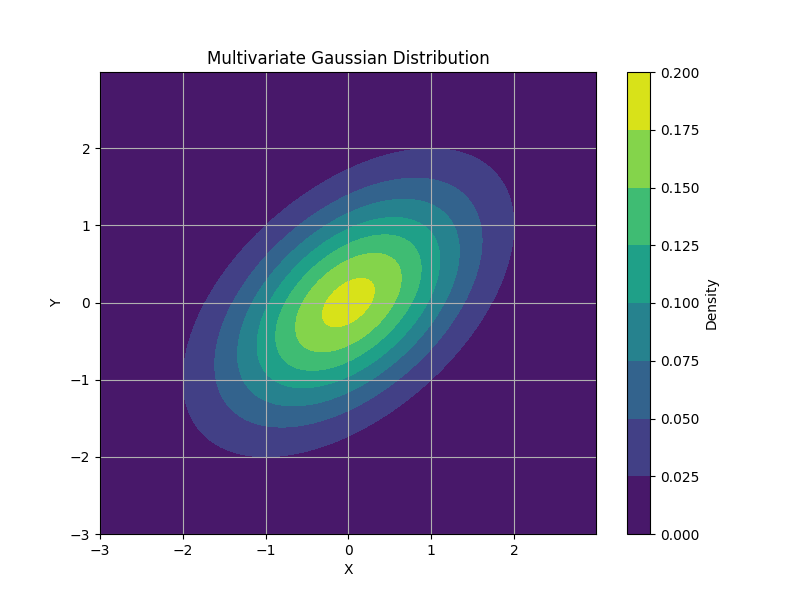
\includegraphics[width=\textwidth]{text/chapter_01/imgs/mvn_contour}
        \caption{Example of multivariate Gaussian distribution - contour plot.}
        \label{fig:mvn_contour}
    \end{subfigure}
    \hfill
    \begin{subfigure}[b]{0.45\textwidth}
        \centering
        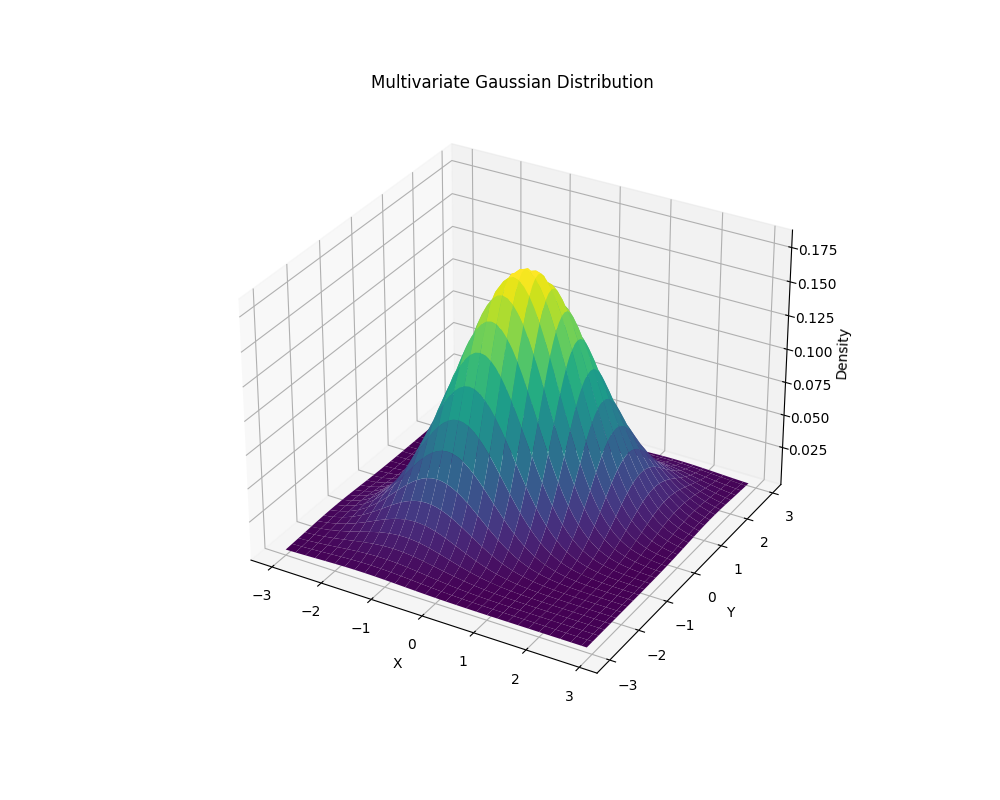
\includegraphics[width=\textwidth]{text/chapter_01/imgs/mvn_3d}
        \caption{Example of multivariate Gaussian distribution - 3D plot.}
        \label{fig:mvn_3d}
    \end{subfigure}
    \caption{Examples of plots of multivariate Gaussian distribution.}
    \label{fig:mvnplot}
\end{figure}

\begin{figure}[htbp]
    \centering
    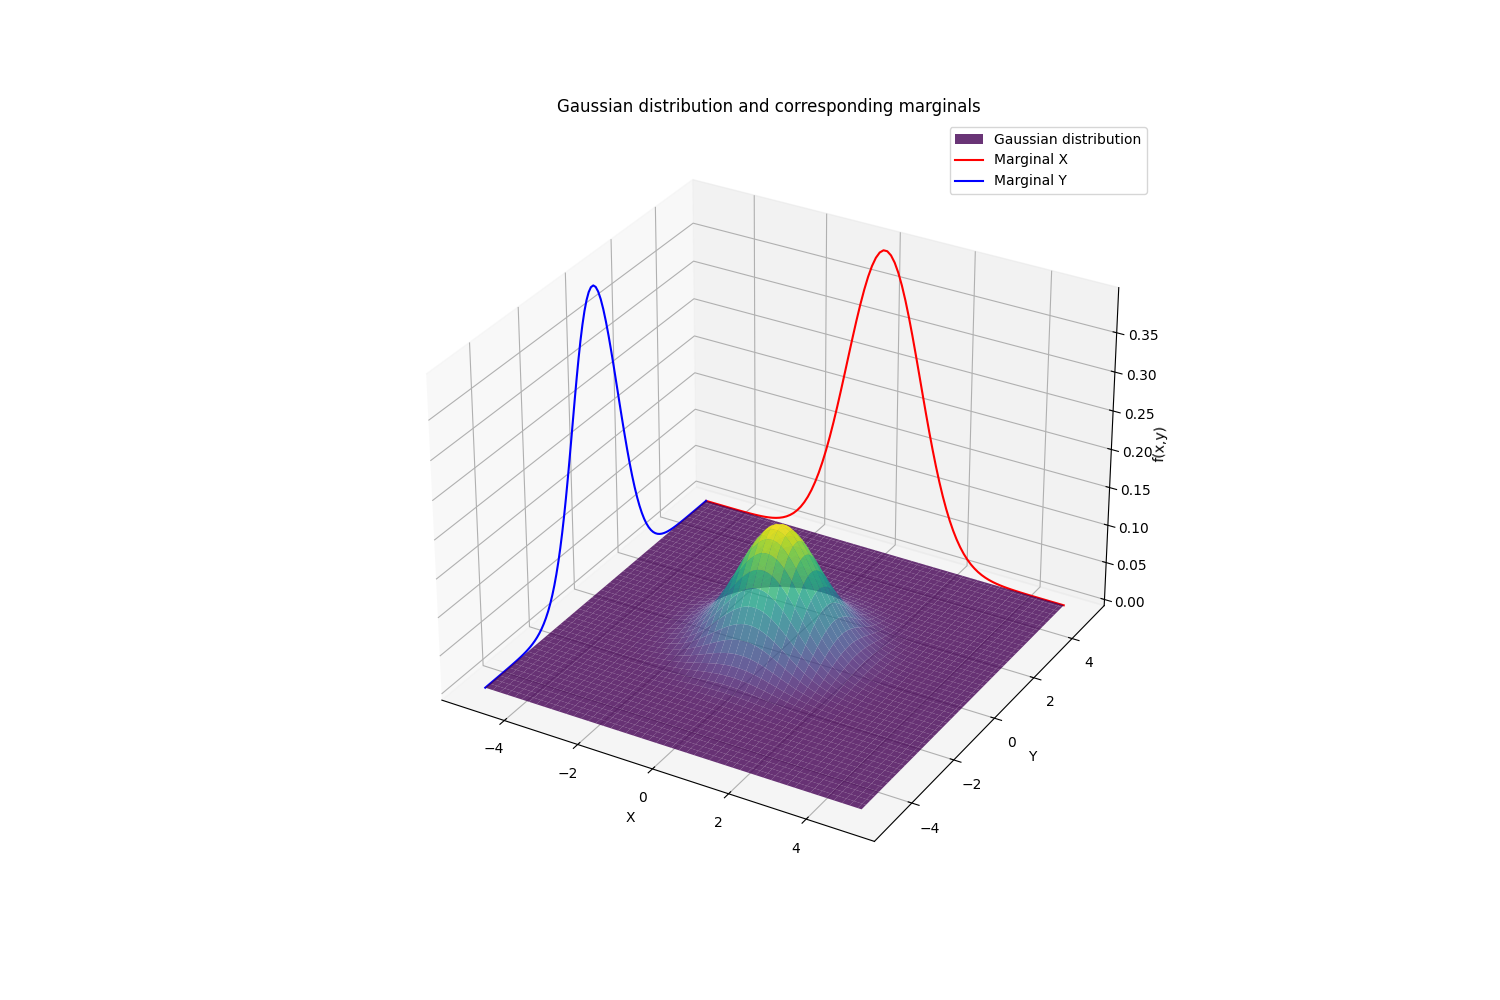
\includegraphics[width=1\textwidth]{text/chapter_01/imgs/gauss_with_marginals}
    \caption{Gaussian distribution with corresponding marginals.}
    \label{fig:gaussWithMarginals}
\end{figure}
    \section{Gaussian mixture}
%A Bayesian Gaussian mixture model is commonly extended to fit a vector of unknown parameters, or multivariate normal
%distributions. In a multivariate distribution, a vector of parameters (such as several observations of a signal) is modeled using a Gaussian mixture model prior distribution on the vector of estimates given by
Gaussian Mixture Models offer a flexible and powerful framework for representing complex probability distributions by combining multiple Gaussian components. In a Gaussian mixture model, a vector of parameters (e.g., observations of a signal) is modeled using a mixture distribution comprising several Gaussian components.
    \begin{align}
        p(\Theta) = \sum_{i=1}^k w_i \mathcal{N}(\mathbf{\mu}_i, \mathbf{\Sigma}_i),
    \end{align}
where the $i^{th}$ vector component is characterized by Gaussian distributions with weights $w_i$, means $\mathbf{\mu}
_i$ and covariance matrices $\mathbf{\Sigma}_i$. These parameters are encapsulated to the parameter $\Theta$ in $p(\cdot)$.

%In multi-target tracking, we are often dealing with linear Gaussian models, thus the posterior density is
%represented as a mixture of one or many Gaussian components. The pdf of Gaussian mixture distribution is simple sum of every Gaussian component, so the formula is as follows:
In the context of multi-target tracking, Gaussian mixture models find utility in capturing the complex nature of target states and measurements. MTT often involves dealing with linear Gaussian models, where the posterior density is represented as a mixture of one or more Gaussian components. This representation enables MTT algorithms to probabilistically model uncertainties associated with target dynamics, sensor measurements, and data association.

The probability density function (pdf) of a Gaussian mixture distribution is a simple sum of each Gaussian component, expressed as
    \begin{align}
        p(x) &= \sum_{i=1}^k w_i\mathcal{N}(\mathbf{x};\mathbf{\mu_i}, \mathbf{\Sigma_i}),
    \end{align}
where $k$ is the number of Gaussian component, $w_i>0$ is the weight of $i^{th}$ component and $\sum_{i=1}^k w_i = 1$.

In MTT, Gaussian mixture models are particularly useful for tasks such as data association, where they probabilistically assign measurements to existing tracks or create new tracks based on the likelihood of observations given the target states. By modeling complex distributions of target states and measurements, Gaussian mixture models enable MTT algorithms to handle uncertainties and ambiguities inherent in real-world tracking scenarios, including occlusions, clutter, and target interactions.

Examples of multivariate Gaussian mixture distribution are shown in Figure \ref{fig:mvn_mixture_plot}. Gaussian mixture distribution with marginal distribution for each dimension in Figure \ref{fig:gaussMixWithMarginals}.
\begin{figure}[htbp]
    \centering
    \begin{subfigure}[b]{0.45\textwidth}
        \centering
        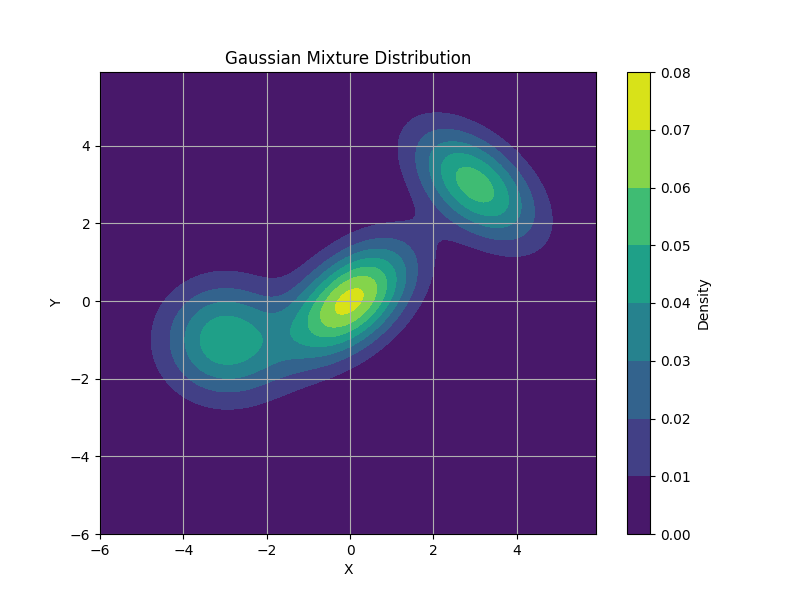
\includegraphics[width=\textwidth]{text/chapter_01/imgs/mvn_mixture_contour}
        \caption{Example of multivariate Gaussian mixture distribution - contour plot.}
        \label{fig:mvn_mixture_contour}
    \end{subfigure}
    \hfill
    \begin{subfigure}[b]{0.45\textwidth}
        \centering
        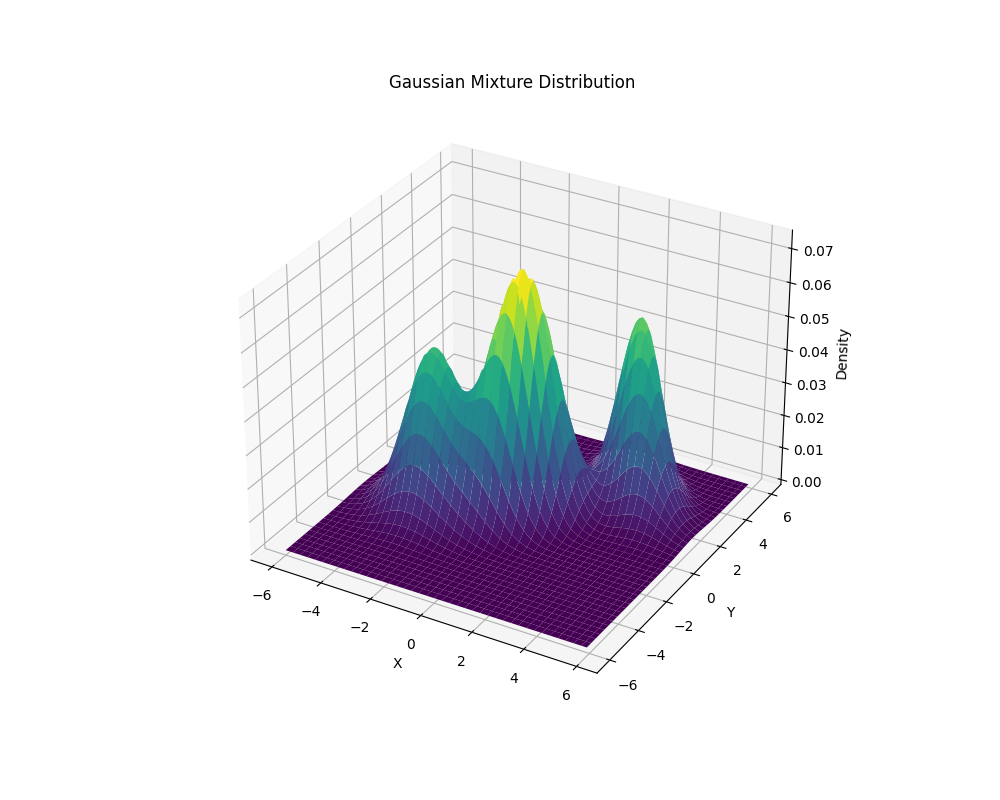
\includegraphics[width=\textwidth]{text/chapter_01/imgs/mvn_mixture_3d}
        \caption{Example of multivariate Gaussian mixture distribution - 3D plot.}
        \label{fig:mvn_mixture_3d}
    \end{subfigure}
    \caption{Examples of plots of multivariate Gaussian mixture distribution. There are three components in figures with means $\{[0, 0], [3, 3], [-3, -1]\}$. Note that the density of peaks is very low, because the sum has to be equal $1$.}
    \label{fig:mvn_mixture_plot}
\end{figure}

\begin{figure}[htbp]
    \centering
    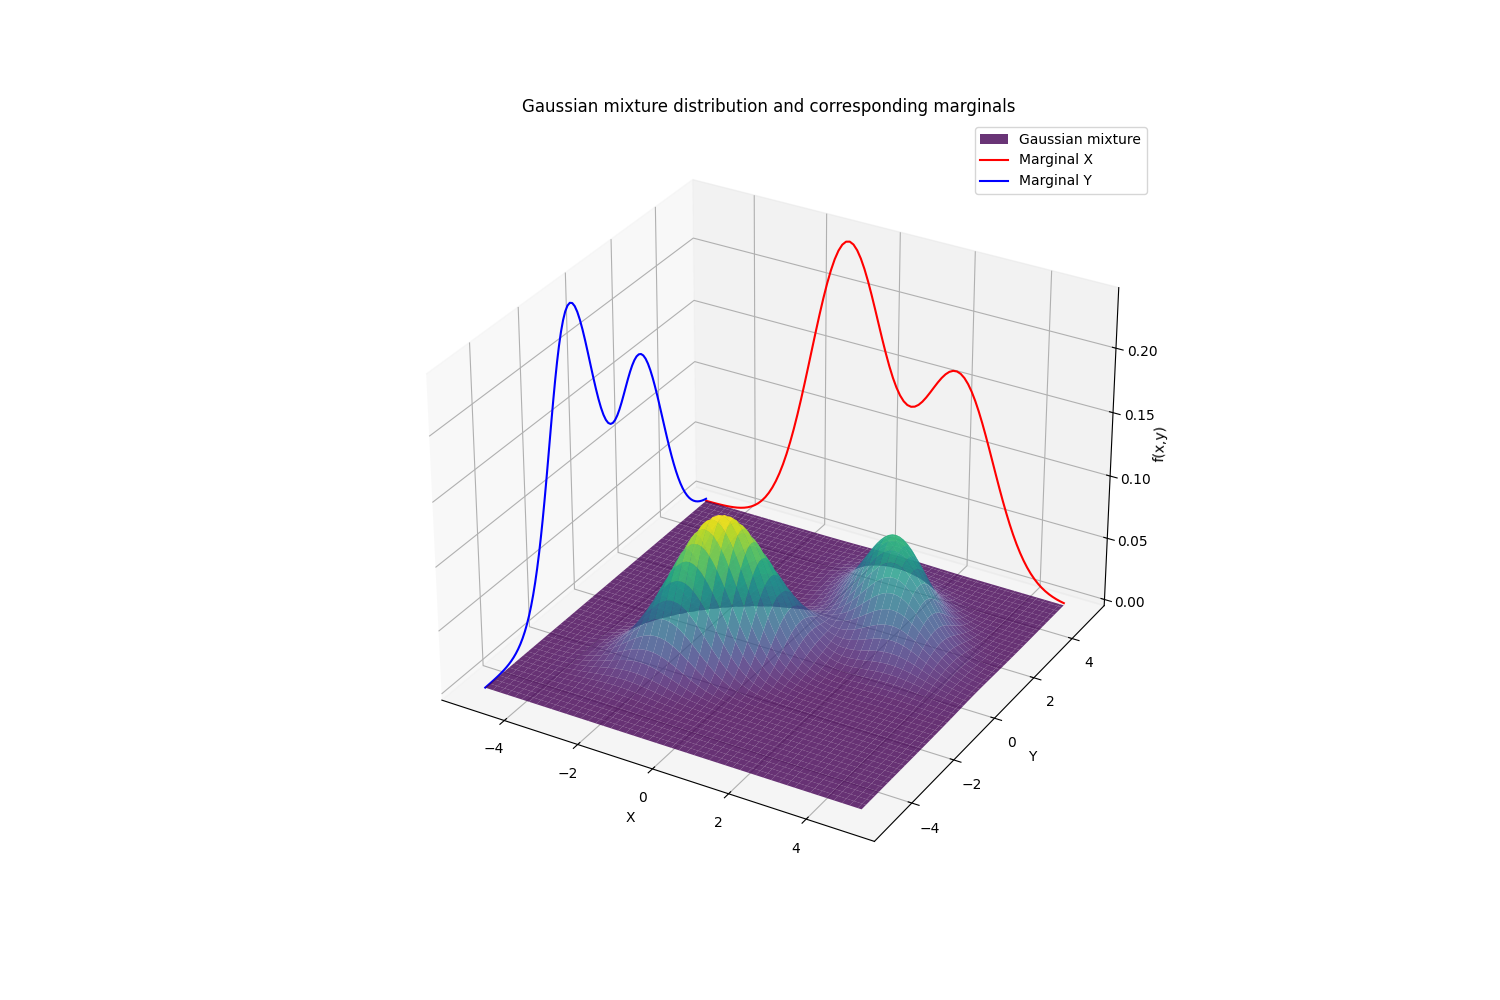
\includegraphics[width=1\textwidth]{text/chapter_01/imgs/gaussMix_with_marginals}
    \caption{Gaussian mixture distribution with means $\{[0,0], [2,2]\}$, weights $\{[0.6, 0.4]\}$ and corresponding marginals.}
    \label{fig:gaussMixWithMarginals}
\end{figure}

    \section{State space model}
\label{sec:stateSpaceModel}
State-space models serve as a fundamental framework for describing the evolution of dynamic systems over time. In the context of multi-target tracking, state-space models provide a formalism for representing motion dynamics of targets and the measurement process, enabling efficient and accurate inference of target states from sensor data.

At the core of a state-space model lies a set of latent variables, known as the state vector, which encapsulates the
unobservable quantities of interest, such as the position, velocity, and acceleration of targets in MTT. The dynamics governing the evolution of the state vector are typically described by a transition model, which specifies how the state evolves over time according to a probabilistic process. This transition model can take various forms depending on the nature of the system dynamics, ranging from simple linear or non-linear models to more complex stochastic processes.

In addition to the transition model, state-space models incorporate an observation model that describes the relationship between the observed measurements and the underlying state variables. This observation model accounts for the uncertainties and noise inherent in the measurement process, allowing for the probabilistic mapping of observed data to the latent state space.

State-space model can be represented as a pair of stochastic equations.
\begin{enumerate}
    \item \textbf{State transition equation:}
        \begin{align}
                  \mathbf{x_k} &= f(\mathbf{x_{k-1}}, \mathbf{u_k}, \mathbf{w_k}), \label{eq:state_space_model_state}
        \end{align}
        where $\mathbf{x_k}$ represents the state vector at time $k, f$ denotes the transition function describing the
        evolution of the state, $\mathbf{u_k}$ represents optional control inputs, and $\mathbf{w_k}$ denotes process
    noise.
    \item \textbf{Observation equation:}
        \begin{align}
            \mathbf{z_k} &= h(\mathbf{x_{k}}, \mathbf{v_k}), \label{eq:state_space_model_observation}
        \end{align}
        where $\mathbf{z_k}$ represents the observed measurements at time $k, h$ denotes the observation function
    mapping the
    state to measurements, and $v_k$ represents the measurement noise.
\end{enumerate}

In MTT, state-space models provide a natural framework for representing the motion dynamics of multiple targets and the sensor measurements associated with each target. Each target is typically associated with its own state vector, allowing for simultaneous tracking of multiple objects within the same probabilistic framework.

State-space models enable MTT algorithms to perform a range of tasks, including target prediction, data association, and state estimation by propagating the state forward in time using the transition model and updating the state based on observed measurements using the observation model. By incorporating uncertainty explicitly into the tracking process, state-space models facilitate robust inference of target states in complex and dynamic tracking scenarios.

While state-space models offer a powerful framework for multi-target tracking, they also present several challenges and considerations.
\begin{itemize}
    \item \textbf{Model complexity:} Designing an appropriate state-space model requires careful consideration of the
    underlying dynamics and measurement process, which can be challenging in complex tracking scenarios with non-linearities and uncertainties.
    \item \textbf{Parameter estimation:} Estimating the parameters of a state-space model from data, such as the transition and observation matrices, can be computationally demanding and prone to issues such as overfitting or underfitting.
    \item \textbf{Computational Complexity:} Performing inference in state-space models often involves recursive algorithms such as the Kalman filter or particle filter, which can be computationally intensive, especially in high-dimensional or real-time tracking applications.
\end{itemize}

Despite these challenges, state-space models remain a cornerstone of multi-target tracking, offering a principled and flexible framework for representing and reasoning about dynamic systems in the presence of uncertainty.
There are many state space models used in MTT. Before we define two of the most common ones in next sections, it
should be noted, that definitions in \eqref{eq:state_space_model_state} and \eqref{eq:state_space_model_observation} are too general, because $f_k$ and $h_k$ could by any functions.

To get a closed-form solution in the Bayesian inference framework, we need
to choose conjugate distributions for the likelihood and the prior. The Kalman filter (see Section \ref{sec:Kalman} for
more) works for the Gaussian-linear case, where the functions
$f_t$ and $h_t$ are linear and noisy variables and are distributed as Gaussians with zero mean. The Gaussian linear
state space model has the formulation:
\begin{align}
    p(x_k|x_{k-1}) &= Fx_{k-1} + Bu_k + w_k
     &w_k \sim \mathcal{N}(0,Q),\\
    p(z_k|x_k) &= Hx_k + v_k
     &v_k \sim \mathcal{N}(0,R), \\
    p(x_0) &\sim \mathcal{N}(\hat{x}_0, P_0),
\end{align}
where
\begin{itemize}
    \item F is the transition matrix of appropriate dimension,
    \item B is the input matrix of appropriate dimension,
    \item H is the measurement matrix of appropriate dimension,
    \item Q is the symmetric positive semi-definite covariance matrix of
    motion noise $
    w_k$,
    \item R is the symmetric positive semi-definite covariance matrix of
    measurement
    noise $v_k$,
    \item $\hat{x}_0$ and $P_0$ are the mean and the covariance matrix of the prior state.
\end{itemize}
The control variable $u_k$, in general, represents some input signal from the environment, and
$B$ specifies how the input signal affects the dynamic system. This variable is ususally not considered in MTT scenarios.
In multi-target tracking, most often with Gaussian linear models is worked, thus following formulation is instead used.
\begin{align}
    p(x_k|x_{k-1}) &= \mathcal{N}(x_k; Fx_{k-1}, Q),  \\
    p(z_k|x_k) &= \mathcal{N}(z_k;Hx_k,R), \\
    p(x_0) &\sim \mathcal{N}(x_0;\hat{x}_o, P_0).
\end{align}


    \subsection{Constant velocity model}
The constant velocity model (CVM) is a fundamental component of multi-target tracking systems, providing a simplified yet effective representation of target motion dynamics over time. This model assumes that the target's velocity remains constant between consecutive time steps, making it particularly suitable for tracking objects with relatively smooth and predictable motion patterns. In this section, we explore the conceptual basis, mathematical formulation, and practical implications of the constant velocity model in the context of MTT.

At its core, the constant velocity model embodies the notion of inertia, where a target maintains a constant velocity unless acted upon by external forces. This conceptual simplicity allows for a straightforward representation of target motion, making the constant velocity model a popular choice for MTT applications where targets exhibit relatively uniform and predictable movement behaviors.

Mathematically, the constant velocity model describes the evolution of a target's state vector over time in terms of
its position and velocity. At each time step $k$, the state vector $\mathbf{x}_k$ comprises the position $[x_{1,k},x_{
    2,k}]$ and velocity $s$ of the target
\begin{align}
    \mathbf{x}_k &= [x_{1,k}, x_{2,k}, s_{1,k}, s_{2,k}]^T.
\end{align}

The dynamics of the constant velocity model can be represented using a state transition matrix $F$  and a process
noise vector $w_k$, where the state transition matrix captures the relationship between the target's state at
consecutive time steps
\begin{align}
    \mathbf{x}_{k+1} &= \mathbf{F x}_k + \mathbf{w}_k.
\end{align}
All together, vector $\mathbf{x}_k$, matrices $\mathbf{F}$ and $\mathbf{Q}$, might, for example, be represented as
\begin{align}
    \mathbf{x}_k &=
        \begin{bmatrix}
            x_{1,k} \\
            x_{2,k} \\
            s_{1,k} \\
            s_{2,k} \\
        \end{bmatrix},
    \quad \mathbf{F} =
        \begin{bmatrix}
            1 & 0 & \Delta & 0 \\
            0 & 1 & 0 & \Delta \\
            0 & 0 & 1 & 0 \\
            0 & 0 & 0 & 1 \\
        \end{bmatrix},
    \quad \mathbf{Q} = q^2
        \begin{bmatrix}
            \frac{\Delta^3}{3} & 0 & \frac{\Delta^2}{2} & 0 \\
            0 & \frac{\Delta^3}{3} & 0 & \frac{\Delta^2}{2} \\
            \frac{\Delta^2}{2} & 0 & \Delta & 0 \\
            0 & \frac{\Delta^2}{2} & 0 & \Delta \\
        \end{bmatrix},
    \label{eq:state_space_model}
\end{align}
where $\Delta$ stands for delta time, i.e., elapsed time between the last estimation and the current one, $q$ is the
motion noise parameter, which represents the uncertainty in the state transition. The measurement model transforms a
state vector from the state space into the measurement space. Since filters derived from Kalman filter assumes only
linear models, the measurement model for CVM assumes the same space as in the state vectors. As a result, the
observation matrix $\mathbf{H}$ and the noise matrix $\mathbf{R}$ can be, with respect to \eqref{eq:state_space_model}, formulated
\begin{align}
    \mathbf{H} &=
    \begin{bmatrix}
        1 & 0 & 0 & 0 \\
        0 & 1 & 0 & 0 \\
    \end{bmatrix},
    \quad \mathbf{R} = r^2
    \begin{bmatrix}
        1 & 0  \\
        0 & 1  \\
    \end{bmatrix},
\end{align}
where $r$ determines the variance of the measurement noise.

To obtain optimal results given by filters, it is essential to set parameters $r$ and $q$ appropriately. There are
three main ways to do it. The first one requires the knowledge of motion noise given by tracked object and the
knowledge of sensor's error when detecting targets, i.e. the noise measurement. This method is often used in
simulations and experiments. The second one is simple trial
and error method with reasonable choices. The last one is using automated methods, like in \cite{BulutEastimation2011}.

In the context of MTT, the constant velocity model serves as a fundamental building block for tracking algorithms,
providing a simplified yet effective representation of a target motion. By assuming the constant velocity, MTT
algorithms
can predict the future positions of targets based on their current state and velocity, facilitating trajectory estimation and target prediction.

One common application of the constant velocity model in MTT is in the design of prediction algorithms, where future positions of targets are estimated based on their current state and velocity information. These predictions are essential for anticipating target movements and facilitating data association, enabling MTT algorithms to maintain track continuity and adapt to changes in target behavior over time.

Moreover, the constant velocity model can be seamlessly integrated into recursive Bayesian filters, such as the Kalman filter, for state estimation in MTT. By incorporating the constant velocity model into the state-space representation of the tracking problem, Kalman filter-based algorithms can effectively fuse measurement information with dynamic predictions to estimate the most likely trajectories of targets over time.
    \subsection{Constant acceleration model}
The Constant Acceleration Model (CAM) stands as a sophisticated extension of the state-space model in multi-target
tracking, offering a more comprehensive representation of target motion dynamics. Unlike simpler models such as the Constant Velocity Model, which assumes a constant velocity for targets over time, the CAM acknowledges the potential for changes in target acceleration, allowing for more accurate and flexible trajectory estimation. This section delves into the conceptual basis, mathematical formulation, and practical implications of the Constant Acceleration Model in the context of MTT.

In MTT scenarios, targets often exhibit varying degrees of acceleration due to factors such as changes in speed,
direction, or environmental influences. Ignoring these accelerative effects can lead to biased trajectory estimates and diminished tracking accuracy. The CAM addresses this limitation by incorporating an additional acceleration component into the state-space model, enabling more faithful representation of target motion dynamics. By accounting for changes in acceleration, the CAM provides MTT algorithms with greater flexibility and adaptability in tracking targets with non-uniform motion profiles.

Mathematically, the Constant Acceleration Model extends the state transition function of the state-space model to
accommodate changes in acceleration over time. At each time step $k$, the evolution of the target's state vector $x_k$ is governed by a set of dynamic equations that describe the position, velocity, and acceleration of the target
\begin{align}
    \mathbf{x}_k &= [x_{1,k}, x_{2,k}, s_{1,k}, s_{2,k}, a_{1,k}, a_{2,k}]^T,
\end{align}
where, as in CVM, $x_{1,k}$, $x_{2,k}$ is the position of an target in two-dimensional space, $s_{1,k}, s_{2,k}$ is
the velocity and $a_{1,k}, a_{2,k}$ are the accelerations in both directions. Matrices $F$ and $Q$ can then be expressed
\begin{align}
    \mathbf{x}_k &=
    \begin{bmatrix}
        x_{1,k} \\
        x_{2,k} \\
        s_{1,k} \\
        s_{2,k} \\
        a_{1,k} \\
        a_{2,k} \\
    \end{bmatrix},
    \quad \mathbf{F} =
    \begin{bmatrix}
        1 & 0 & \Delta & 0 & \frac{1}{2}\Delta^2 & 0\\
        0 & 1 & 0 & \Delta & 0 & \frac{1}{2}\Delta^2\\
        0 & 0 & 1 & 0 & 0 & 0\\
        0 & 0 & 0 & 1 & 0 & 0\\
        0 & 0 & 0 & 0 & 1 & 0\\
        0 & 0 & 0 & 0 & 0 & 1\\
    \end{bmatrix},
    \quad \mathbf{Q} = q^2
    \begin{bmatrix}
        \frac{\Delta^4}{4} & 0 & \frac{\Delta^3}{3} & 0 & \frac{\Delta^2}{2} & 0\\
        0 & \frac{\Delta^4}{4} & 0 & \frac{\Delta^3}{3} & 0 & \frac{\Delta^2}{2}\\
        \frac{\Delta^3}{3} & 0 & \frac{\Delta^2}{2} & 0 & \Delta & 0\\
        0 & \frac{\Delta^3}{3} & 0 & \frac{\Delta^2}{2} & 0 & \Delta \\
        \frac{\Delta^3}{3} & 0 & \frac{\Delta^2}{2} & 0 & \Delta & 0\\
        0 & \frac{\Delta^3}{3} & 0 & \frac{\Delta^2}{2} & 0 & \Delta \\
    \end{bmatrix}.
\end{align}
The measurement model remains unchanged from the standard state-space model, relating the observed measurements $\mathbf{z}_k$ to the target's true state $\mathbf{x}_k$ through a measurement function $h(\cdot)$ corrupted by measurement noise $v_t$
\begin{align}
    \mathbf{H} &=
    \begin{bmatrix}
        1 & 0 & 0 & 0 & 0 & 0 \\
        0 & 1 & 0 & 0 & 0 & 0 \\
    \end{bmatrix},
    \quad \mathbf{R} = r^2
    \begin{bmatrix}
        1 & 0  \\
        0 & 1  \\
    \end{bmatrix},
\end{align}
The Constant Acceleration Model offers several practical advantages in MTT applications:
\begin{itemize}
    \item Improved trajectory estimation: By accounting for changes in acceleration, the CAM enables more accurate
    and realistic trajectory estimation, particularly for targets exhibiting non-uniform motion patterns or sudden changes in velocity.
    \item Enhanced predictive capability: The inclusion of acceleration dynamics allows MTT algorithms to make more
    informed predictions about future target states, improving tracking performance and reducing prediction errors.
    \item Robustness to dynamic environments: In dynamic environments with varying levels of congestion, obstacles,
    or traffic patterns, the CAM provides MTT algorithms with greater robustness and adaptability, enabling effective tracking even in challenging scenarios.
    \item Applications in autonomous systems: In autonomous systems such as self-driving cars, drones, or robotics,
    the CAM plays a crucial role in motion planning, obstacle avoidance, and trajectory prediction, enhancing the safety and efficiency of autonomous navigation.
\end{itemize}
In summary, the Constant Acceleration Model represents a significant advancement in multi-target tracking, offering a
more nuanced and comprehensive approach to modeling target motion dynamics. By incorporating acceleration effects
into the tracking process, the CAM enables MTT algorithms to achieve higher accuracy, robustness, and predictive capability, making it an indispensable tool for a wide range of applications.

    \section{Hidden Markov Model}
In the domain of multi-target tracking, the Hidden Markov Model (HMM) serves as a framework for
capturing the temporal dynamics of target behavior in complex environments. Building upon the principles of Markov
processes, the HMM extends the state-space model by introducing hidden states that govern the evolution of observable
measurements over time. Markov process of the first order is a model, in which current state depends only on the
previous state
\begin{align}
    p(x_k|x_1,\dots,x_{k-2},x_{k-1}, z_1, \dots, z_{k-2}, z_{k-1}) = p(x_k|x_{k-1}) &\quad \text{(transition
    probability)}, \\
    p(z_k|x_1,\dots,x_{k-2},x_{k-1}, x_k, z_1, \dots, z_{k-2}, z_{k-1}) = p(z_k|x_{k}) &\quad \text{(observation
    likelihood)}, \\
    p(x_0)& \quad \text{(initial state)}.
\end{align}
In models of higher order, the transition probability is
\begin{align}
    p(x_k|x_{k-1},\dots,x_{k-n}),
\end{align}
where $n$ is the number of the order. Details of this model is not described in this work and can be seen in \cite{
    HadarHMMHigherOrder}.

In cases where the process is not didectly observable, but can be observed through another observable variable $z_k$,
we often talk about Hidden Markov process.
\begin{figure}[h]
    \centering
    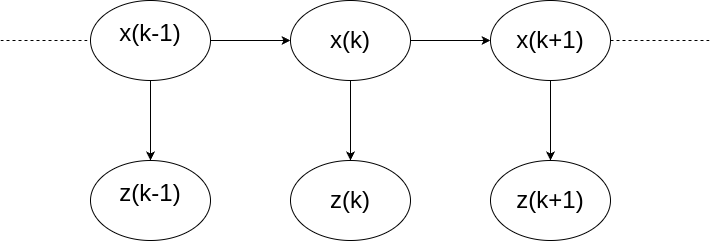
\includegraphics[width=0.8\linewidth]{./text/chapter_01/imgs/HMM}
    \caption{Demonstration of the course of the hidden Markov process.}
    \label{fig:hmm}
\end{figure}

At its core, the Hidden Markov Process represents a stochastic process characterized by a set of hidden states that transition probabilistically over time. While these hidden states are unobservable, they influence the generation of observable measurements, which are assumed to be conditionally independent given the hidden states. In the context of MTT, the hidden states may represent latent attributes of targets, such as their locations, velocities, or motion patterns, while the observable measurements correspond to sensor readings or detections obtained from surveillance systems.

\section{Bayes' filter}
The Bayes filter is a recursive framework that estimates an internal state of the system over time using measurements. The Bayes filter leverages both motion and measurement models, operating under the assumption that these models
accurately describe the system's behavior. Operating within a recursive framework, the Bayes filter continually
estimates the internal state of the system over time using available measurements. Each iteration of the filter
entails two fundamental steps: prediction and update. During the prediction step, the filter anticipates the internal
state $x_k$ based on the preceding state $x_{k-1}$ and the motion model $p(x_k|x_{k-1})$. This prediction step is
commonly referred to as the Chapman-Kolmogorov equation \cite{DedeciusSeq2017}.
\begin{theorem}[The Chapman-Kologorov equation prediction step]
    Given the set of measurements $z_{0:k-1} = {z_0,\dots, z_{k-1}}$, set of control variables $u_{0:k-1} = {u_0,\dots, u_{k-1}}$ and current state $x_{k-1}$ and the motion model $p(x_k|x_{k-1})$, the prediction step is as follows:
    \begin{align}
        p(x_k|z_{0:t-1}, u_{0:k}) &= \int p(x_k|x_{k-1}, u_k) p(x_{k-1}|z_{0:k-1}, u_{0:k-1}) dx_{k-1},
        \label{eq:chapman_kolmogorov_predict}
    \end{align}
    where the integral is taken over the entire state space of $x_{k-1}$, and $p(x_{k-1}|z_{0:k-1}, u_{0:k-1})$ is
    the posterior density of the state at time $k-1$.
\end{theorem}
On the update step, the Bayes' filter corrects (updates) the prediction step with measurements $z_k$ using the
measurement model $p(z_k|x_k)$. This step uses common Bayes' rule.
\begin{theorem}[The update step of Bayes' filter]
    Given the output of Bayes' filter's prediction step, the measurements $z_k$ observed at time $k$ and the
    measurement model $p(z_k|x_k)$, the update step of Bayes' filter is formulated as follows:
    \begin{align}
        \label{eq:bayes_update}
        p(x_k|z_{0:t}, u_{0:t}) &= \frac{p(z_k|x_k) p(x_k|z_{0:k-1},u_{0:k})}{p(z_k|z_{0:k-1})} \propto p(z_k|x_k) p
        (x_k|z_{0:k-1},u_{0:k})
    \end{align}
\end{theorem}
These two steps work in an iterative method, where, in each iteration, first prediction step is used to predict
the state $x_k$ and then update step is used to correct our guess with provided measurement.
\section{Kalman filter}
    \label{sec:Kalman}
The Kalman filter, named after its developer Rudolf E. Kalman, has a rich history dating back to the early 1960s when Kalman first introduced the algorithm in a series of landmark papers. Initially developed for aerospace applications, the Kalman filter gained prominence for its ability to provide optimal state estimation in the presence of noisy measurements and uncertain dynamics.

Over the years, the Kalman filter has found widespread usage across diverse fields and industries, including aerospace, robotics, finance, and telecommunications. Its applications range from tracking spacecraft trajectories and guiding missiles to monitoring financial markets and controlling autonomous vehicles. The filter's versatility, efficiency, and effectiveness have made it a cornerstone of modern estimation and control systems.

The Kalman filter operates on the principles of recursive Bayesian estimation, utilizing a system dynamics model and noisy measurements to predict and update the state of a dynamic system over time. Its mathematical elegance and simplicity make it well-suited for real-time applications, enabling accurate and efficient state estimation even in complex and uncertain environments.

Despite its remarkable success, the Kalman filter continues to evolve, with extensions and variations such as the
extended Kalman filter (EKF), unscented Kalman filter (UKF), and particle filter (PF) addressing more challenging scenarios involving non-linear dynamics and non-Gaussian noise.

In summary, the Kalman filter stands as a seminal contribution to the field of estimation and control, with a rich history of development and widespread usage across diverse domains. Its continued relevance and versatility underscore its status as a foundational tool for state estimation and tracking in modern technological applications.

\subsection{Kalman filter inference}
In Section \ref{sec:stateSpaceModel} we talked about state space model, which is used by Kalman filter. Thus we work
with equations
\begin{align}
    x_k &= Fx_{k-1} + w_t \\
    z_t &= Hx_k + v_k,
\end{align}
where both noise variables are independent and with zero mean
\begin{align}
    w_k &\sim \mathcal{N}(0,Q), \\
    v_k &\sim \mathcal{N}(0,R).
\end{align}
Then the state and measurement distributions follows
\begin{align}
    x_k &\sim \mathcal{N}(Fx_{k-1},Q) \qquad && \text{with density}\quad p(x_k|x_{k-1}), \\
    z_k &\sim  \mathcal{N}(Hx_k,R) \qquad && \text{with density}\quad p(z_k|x_k).
\end{align}
Because Kalman filter is Bayesian, we need prior distribution for $x_k$. Model $z_k$ is Gaussian, conjugate prior and
is then also Gaussian with mean $x_{k-1}^+$ and covariance matrix $P_{k-1}^+$,
\begin{align}
    p(x_k|z_{0:k-1}) &= \mathcal{N}(x_{k-1}^+,P_{k-1}^+).
\end{align}

The prediction step is derived from Formula (\ref{eq:chapman_kolmogorov_predict}). Note, that by multiplicating two
Gaussian distributions we again get Gaussian distribution $\mathcal{N}(x_k^-,P_k^-)$ with hyperparemeters
\begin{align}
    x_k^- &= Fx_{k-1}^+ \\
    P_k^- &= FP_{k-1}^{+}F^T + Q.
\end{align}
By multiplicating two Gaussian distributions followed by marginalization, we enumerate the state equation. The
estimation
of state $x_k^-$ is just applying model variables into appropriate equations. The estimated covariance $P_k^-$
expresses the degree of uncertainty of the estimation. By applying this step, the uncertainty grows.

The update step corrects the prediction step by applying new observed measurements $z_k$. For that, formula (\ref{eq:bayes_update}) is used. The model is transformed into exponential form
\begin{align}
    p(z_k|x_k) &\propto \exp \left\{-\frac{1}{2}(z_k - Hx_k)^T R^{-1} (z_k - Hx_k)\right \} \nonumber \\
    &= \exp
    \left\{
        Tr\left(
        \underbrace{
            -\frac{1}{2}
            \begin{bmatrix}
                -1 \\
                x_k
            \end{bmatrix}
            \begin{bmatrix}
                -1 \\
                x_k
            \end{bmatrix}^T
        }_{\eta}
        \underbrace{
            \begin{bmatrix}
                z_k^T \\
                H^T
            \end{bmatrix}
            R^{-1}
            \begin{bmatrix}
                z_k^T \\
                H^T
            \end{bmatrix}^T
        }_{T(z_k)}
        \right)
    \right\}.
\end{align}
The conjugated shape has the form
\begin{align}
    p(x_k|z_{0:k-1}) &\propto \exp
    \left\{-\frac{1}{2}(x_k - x_k^-)^T (P_k^-)^{-1} (x_k - x_k^-)\right \} \nonumber \\
    &= \exp
    \left\{
    Tr\left(
    \underbrace{
        -\frac{1}{2}
        \begin{bmatrix}
            -1 \\
            x_k
        \end{bmatrix}
        \begin{bmatrix}
            -1 \\
            x_k
        \end{bmatrix}^T
    }_{\eta}
    \underbrace{
        \begin{bmatrix}
            (x_k^-)^T \\
            I
        \end{bmatrix}
        (P_k^-)^{-1}
        \begin{bmatrix}
            (x_k^-)^T \\
            I
        \end{bmatrix}^T
    }_{\xi_k}
    \right)
    \right\},
\end{align}
where $I$ is identity matrix of appropriate shape.

The bayesian update is a sum of the hyperparameter and sufficient statistic,
\begin{align}
    \xi_{k}
    &= \xi_{k-1} +  T(z_{k})  \nonumber \\
    &=
    \begin{bmatrix}
    (x_{k}^{-})^{T} (P_{k}^{-})^{-1} x_{k}^{-} + z_{k}^{T} R^{-1} z_{k},
    & (x_{k}^{-})^{T} (P_{k}^{-})^{-1} + z_{k}^{T} R^{-1} H \\
    (P_{k}^{-})^{-1} (x_{k}^{-})^{T} + H^{T} R^{-1} z_{k},
    & (P_{k}^{-})^{-1} + H^{T} R^{-1} H.
    \end{bmatrix}
\end{align}
The posterior parameters are then derived
\begin{align}
    P_{k}^{+} &= (\xi_{k;[2,2]})^{-1} \notag\\
    &= \left[ (P_{k}^{-})^{-1} + H^{T} R^{-1} H \right]^{-1} \notag\\
    &= (I - K_{k} H) P_{k}^{-} \\
    x_{k}^{+} &= (\xi_{k;[2,2]})^{-1} \xi_{k;[2,1]} \notag\\
    &= P_{k}^{+} \left[ (P_{k}^{-})^{-1} (x_{k}^{-})^{T} + H^{T} R^{-1} z_{k}\right] \notag \\
    &= x_{k}^{-} + P_{k}^{+} H^{T} R^{-1}(z_{k} - Hx_{k}^{-}),
\end{align}
where
\begin{align}
    K_{k} &= P_{k}^{-} H^{T}(R + H P_{k}^{-}H^{T})^{-1} \label{eq:kalman_gain}
\end{align}
is the Kalman gain. This form is the optimal Kalman gain, as it minimizes the root mean squared error. In general, the
greater the gain, the greater the emphasis of the new measurements. The filter is then more sensitive.

There are several possible formulas that express the optimal Kalman filter. One of the most popular formulations is
as follows:
\begin{align}
    \hat{z}_{k}^{-} &= H \hat{x}_{k}^{-}, \qquad &&\text{(measurement prediction)} \\
    \nu_t &= z_t - \hat{z}_{k}^{-}, \qquad &&\text{(innovation or prediction error $z_t$)} \\
    S_t &= H P_{k}^{-} H^T + R, \qquad &&\text{(covariance of innovation $\nu_t$)} \\
    K_t &= P_{k}^{-} H^T S_t^{-1}, \qquad &&\text{(Kalman gain)} \\
    {x}_{k}^{+} &= \hat{x}_{k}^{-} + K_t \nu_t, \qquad &&\text{(posterior state estimation $x_t$)} \\
    P_{k}^{+} &= (I - K_t H) P_{k}^{-}. \qquad &&\text{(posterior covariance)}
\end{align}

The pseudo-algorithm of Kalman filter is shown in Algorithm \ref{alg:kalman_filter}.
\begin{algorithm}
    \caption{Kalman Filter Algorithm}
    \begin{algorithmic}[1]
        \State \textbf{Inputs:} Initial state estimate $\hat{x}_0$, initial covariance matrix $P_0$, system
        dynamics matrix $F$, process noise covariance matrix $Q$, measurement matrix $H$, measurement noise
        covariance matrix $R$, and measurements $Z$.
        \State \textbf{Outputs:} Updated state estimate $\hat{x}_k$ and updated covariance matrix $P_k$.
        \State
        \Procedure{Initialization}{$x_0,P$}
            \State $\hat{x}_0 = x_0$  \Comment{Initialize state estimate}
            \State $P_0 = P$ \Comment{Initialize error covariance matrix}
        \EndProcedure

        \State
        \Procedure{Prediction step}{}
            \State $\hat{x}_{k|k-1} = F \hat{x}_{k-1} $ \Comment{Predict state estimate}
            \State $P_{k|k-1} = F P_{k-1} F^T + Q$ \Comment{Predict covariance:}
        \EndProcedure

        \State
        \Procedure{Update step}{$z_k$}
            \State $K_k = P_{k|k-1} H^T (H P_{k|k-1} H^T + R)^{-1}$ \Comment{Kalman gain}
            \State $\hat{x}_k = \hat{x}_{k|k-1} + K_k(z_k - H \hat{x}_{k|k-1})$ \Comment{Update state estimate}
            \State $P_k = (I - K_k H) P_{k|k-1}$ \Comment{Update covariance}
        \EndProcedure
        \State
        \Procedure{Kalman filter recursion}{}
            \State Initialization
            \ForAll{z_k $ \in$ Z}
                \State Perform Prediction Step
                \State Perform Update Step with $z_k$
            \EndFor
        \EndProcedure

    \end{algorithmic}
    \label{alg:kalman_filter}
\end{algorithm}